%% Spec Manager paper — SIGGRAPH / ACM TOG submission draft.
%% Build: latexmk -pdf main.tex
%%
%% Submission format: [acmtog,review,anonymous]. For camera-ready switch to
%% \documentclass[acmtog]{acmart}. For a quick conference-style preview use
%% [manuscript,screen,review]{acmart} as suggested by the acmart sample.

\RequirePackage{xurl} % breakable URLs; must load before acmart's hyperref
\documentclass[acmtog,review,anonymous]{acmart}

%% ------------------------------------------------------------------ %%
%% Markers for unfinished content. Every \RESULT must be replaced by an
%% experiment-produced number before any draft leaves the repo.
\newcommand{\TODO}[1]{\textcolor{red}{[TODO: #1]}}
\newcommand{\RESULT}[1]{\textcolor{red}{[RESULT: #1]}}
%% ------------------------------------------------------------------ %%

\usepackage{booktabs}
\usepackage{xcolor}

%% ------------------------------------------------------------------ %%
%% Overfull \hbox control. acmart already loads microtype; the two knobs
%% below let TeX relax a line by a little interword stretch instead of
%% pushing a long, unbreakable term past the column edge. This is NOT
%% \sloppy -- justification stays tight everywhere else.
\emergencystretch=2em
\hyphenation{
  un-der-spe-ci-fi-ca-tion
  un-der-spe-ci-fied
  Con-firmed-Value-Miss-ing
  Un-sup-por-ted-Lit-er-al
}

%TC:beginignore
\AtBeginDocument{%
  \providecommand\BibTeX{{Bib\TeX}}}
%TC:endignore

%% CCS concepts: generate the authoritative strings with the ACM tool at
%% https://dl.acm.org/ccs before submission; these are provisional.
\ccsdesc[500]{Computing methodologies~Shape modeling}
\ccsdesc[300]{Computing methodologies~Natural language generation}
\ccsdesc[300]{Computing methodologies~Software verification and validation}
\ccsdesc[100]{Human-centered computing~Interactive systems and tools}

%% Authors: anonymized for review. Fill from the migration repo metadata.
\author{Anonymous Author(s)}
\affiliation{\institution{Anonymous Institution}\city{}\country{}}

\begin{document}

\title{Grounded Before Drawn: Provenance-Tracked Specifications and
  Ground-Truth-Free Verification for Text-to-CAD Agents}

\begin{abstract}
Proactive clarification has recently entered text-to-CAD pipelines: a
clarifier detects underspecified or conflicting prompts and asks questions
before a coder generates executable CAD programs. Yet these pipelines still
rely on a single free-text handoff between agents, with no explicit
mechanism to trace information lost or assumptions introduced during the
process. We introduce a \emph{Spec Manager} that replaces this handoff with
a provenance-tracked design specification: a graph of features, parameters,
and constraints in which every value is attributed to the user's prompt, a
clarification answer, a system assumption, or a derived constraint. A
deterministic kernel governs specification updates, applies explicit
conflict policies, and detects unresolved fields, making specification
invariants auditable and unit-testable without an API call.

We further introduce a two-channel, spec-grounded verifier that checks
generated programs against the specification without requiring
ground-truth geometry at inference time. Its static channel parses the
program, maps CAD operations and parameters to specification fields, and
checks confirmed values and parameter provenance; mappings it cannot
establish reliably are reported as uncertain rather than silently passed.
Its dynamic channel measures the executed B-rep---including dimensions,
radii, depths, and feature counts---to detect geometric violations that
static analysis cannot establish. Verification outcomes trigger targeted
responses: unresolved assumptions are returned to the user as clarification
questions, while confirmed requirements omitted or violated by the coder
trigger diagnostic-grounded regeneration.

On a controlled recreation of the ProCAD misleading-prompt benchmark,
free-text handoffs exhibit information defects in \RESULT{C1 defect rate}
of clarified samples. Our specification pipeline reduces this rate to
\RESULT{C2 defect rate}, improves mean Chamfer distance from
\RESULT{baseline CD} to \RESULT{our CD} under equal or smaller question
budgets, and predicts ground-truth geometric failures with
\RESULT{precision/recall}. We also show that the Spec Manager can be
distilled into Qwen2.5-7B with kernel-canonicalized labels. Together,
these results provide evidence that specification fidelity is a measurable
inference-time signal for geometric correctness, while ground-truth metrics
remain an offline evaluation tool.
\end{abstract}

\keywords{text-to-CAD, multi-agent systems, design specification, provenance,
program verification, Clarifier--Coder pipelines}

\maketitle

\section{Introduction}\label{sec:intro}

Text-to-CAD systems turn natural-language descriptions into executable
parametric programs---typically CadQuery or construction-sequence code that is
rendered into boundary-representation (B-rep) geometry
\cite{deepcad,text2cad,llm4cad,cadrecode}. The promise is a conversational
interface to mechanical design; the reality is that users' descriptions are
almost always incomplete, occasionally self-contradictory, and rarely stated
at the level of precision a parametric program requires. Recent work addresses
this with \emph{proactive clarification}: an agent interrogates the prompt
before a second agent writes code \cite{procad}. ProCAD demonstrates that a
single round of questions, answered by an oracle user simulator, can recover
much of the geometry lost to underspecified or conflicting prompts.

Yet the two agents in this pipeline never share structured state. Their
\textbf{only hand-off is a single piece of free text}---a rewritten
``standardized prompt'' produced by the clarifier. Whatever the
question--answer exchange drops or invents is invisible to the coder;
whatever the coder ignores or improvises is invisible to everyone. There is
no execution-time feedback path either: generated code is evaluated only
offline, against ground-truth meshes that do not exist when the system is
deployed.

That this is not merely an aesthetic concern is suggested by two recent
findings from complementary angles. In verification-driven code generation,
vision--language models that inspect renders of their own CAD output can
catch some geometric errors iteratively \cite{cadcodeverify}---but their
validation questions and answers are both produced by the same model looking
at an image, with no grounded reference to what the user actually confirmed.
On the human side, Treellis \cite{treellis} shows that exposing the
\emph{structure} of a generated model lets users edit locally instead of
regenerating the whole object---yet only \textbf{32 of 50} generated models
were in an editable state on the first pass (43 after adding exemplars and
structural constraints). Exposing structure helps; the structure itself
remains ungrounded and unverified.

We argue that the missing object in this pipeline is a
\emph{provenance-tracked specification of design intent}, sitting between the
user and the coder: a structured feature graph in which every parameter
records \emph{where it came from}---stated by the user, confirmed in a
clarification answer, silently assumed by the system, or derived from a
constraint---and against which the generated program can be checked
\emph{without any ground-truth geometry}. Concretely, we introduce a
\textbf{Spec Manager} agent and a deterministic \textbf{spec-grounded
verifier}, and close the loop between them
(Figure~\ref{fig:overview}):

\begin{enumerate}
  \item \textbf{Structured, provenance-tagged specification
  (\S\ref{sec:spec}).} Instead of a rewritten prompt, the Spec Manager
  maintains a graph of features, parameters, and constraints. Clarification answers
  override earlier statements under an explicit provenance ranking; every
  override is logged in a machine-readable change record. Parameters the
  model fills in without user support are marked as assumptions rather than
  silently inserted. A deterministic kernel---not the LLM---owns merging,
  conflict resolution, and the detection of unresolved fields, so these
  invariants are unit-testable without an API call.

  \item \textbf{Ground-truth-free verification at deployment time
  (\S\ref{sec:verifier}).} The verifier aligns generated CadQuery code back
  to the \emph{specification the user confirmed}, not to a reference mesh. A
  static layer parses the program without executing it, maps its operations
  to specification fields, and flags confirmed values without a reliable
  mapping, dimensional literals with no source in the specification, and
  assumed values realized in code; a dynamic layer
  measures the executed B-rep directly (radii, depths, feature counts,
  topology) to catch the failure class numeric matching cannot---correct
  values with wrong operations, such as a hole that became a boss.

  \item \textbf{A closed loop with differential routing and a question
  budget (\S\ref{sec:loop}).} A missing \emph{assumption} is routed back to
  the user as a targeted question; a confirmed value the coder dropped is
  routed forward with a field-level diagnostic for grounded re-generation---
  the user is never re-asked what they already said. Triggered only on
  demand, the loop is designed to improve geometry under the same or smaller
  question budget than an unconditionally extra clarification round.
\end{enumerate}

We further show the behavior is reproducible without a proprietary model: the
Spec Manager distills into Qwen2.5-7B with training targets canonicalized by
the deterministic kernel, so the student cannot learn malformed schemas from
the teacher (\S\ref{sec:training}).

In a controlled re-creation of the ProCAD benchmark---underspecification and
direct-conflict prompts with severity $K{=}1..3$---we find that free-text
hand-offs lose or invent information in \RESULT{C1 rate} of clarified
samples, that such defects correlate with degraded Chamfer distance
(\RESULT{correlation}), and that the provenance specification reduces them to
\RESULT{C2 rate} while improving mean Chamfer distance from
\RESULT{E1 CD} to \RESULT{E3 CD} at \RESULT{rounds} average questions.
Crucially, verifier verdicts predict ground-truth geometric failure with
\RESULT{precision\slash recall}, establishing the deployment-time signal as a valid
proxy; and under imperfect (noisy or wrong) user answers---conditions the
oracle-simulator evaluation cannot examine---our pipeline degrades more
gracefully (\RESULT{C6 numbers}).

The central conceptual move is a separation the current literature conflates:
\emph{specification fidelity} (does the program realize what the user
confirmed?) from \emph{geometric similarity} (does the output resemble a
reference mesh?). Similarity needs ground truth and is available only in
evaluation; fidelity can be measured every time the system runs. Treellis
gives humans an editable geometric tree after generation; we give the agents a
grounded, traceable intent graph before generation and the means to check it
afterward---making an editable tree for people and a verified specification
for agents natural complements rather than competitors.

\begin{figure}[t]
  \centering
  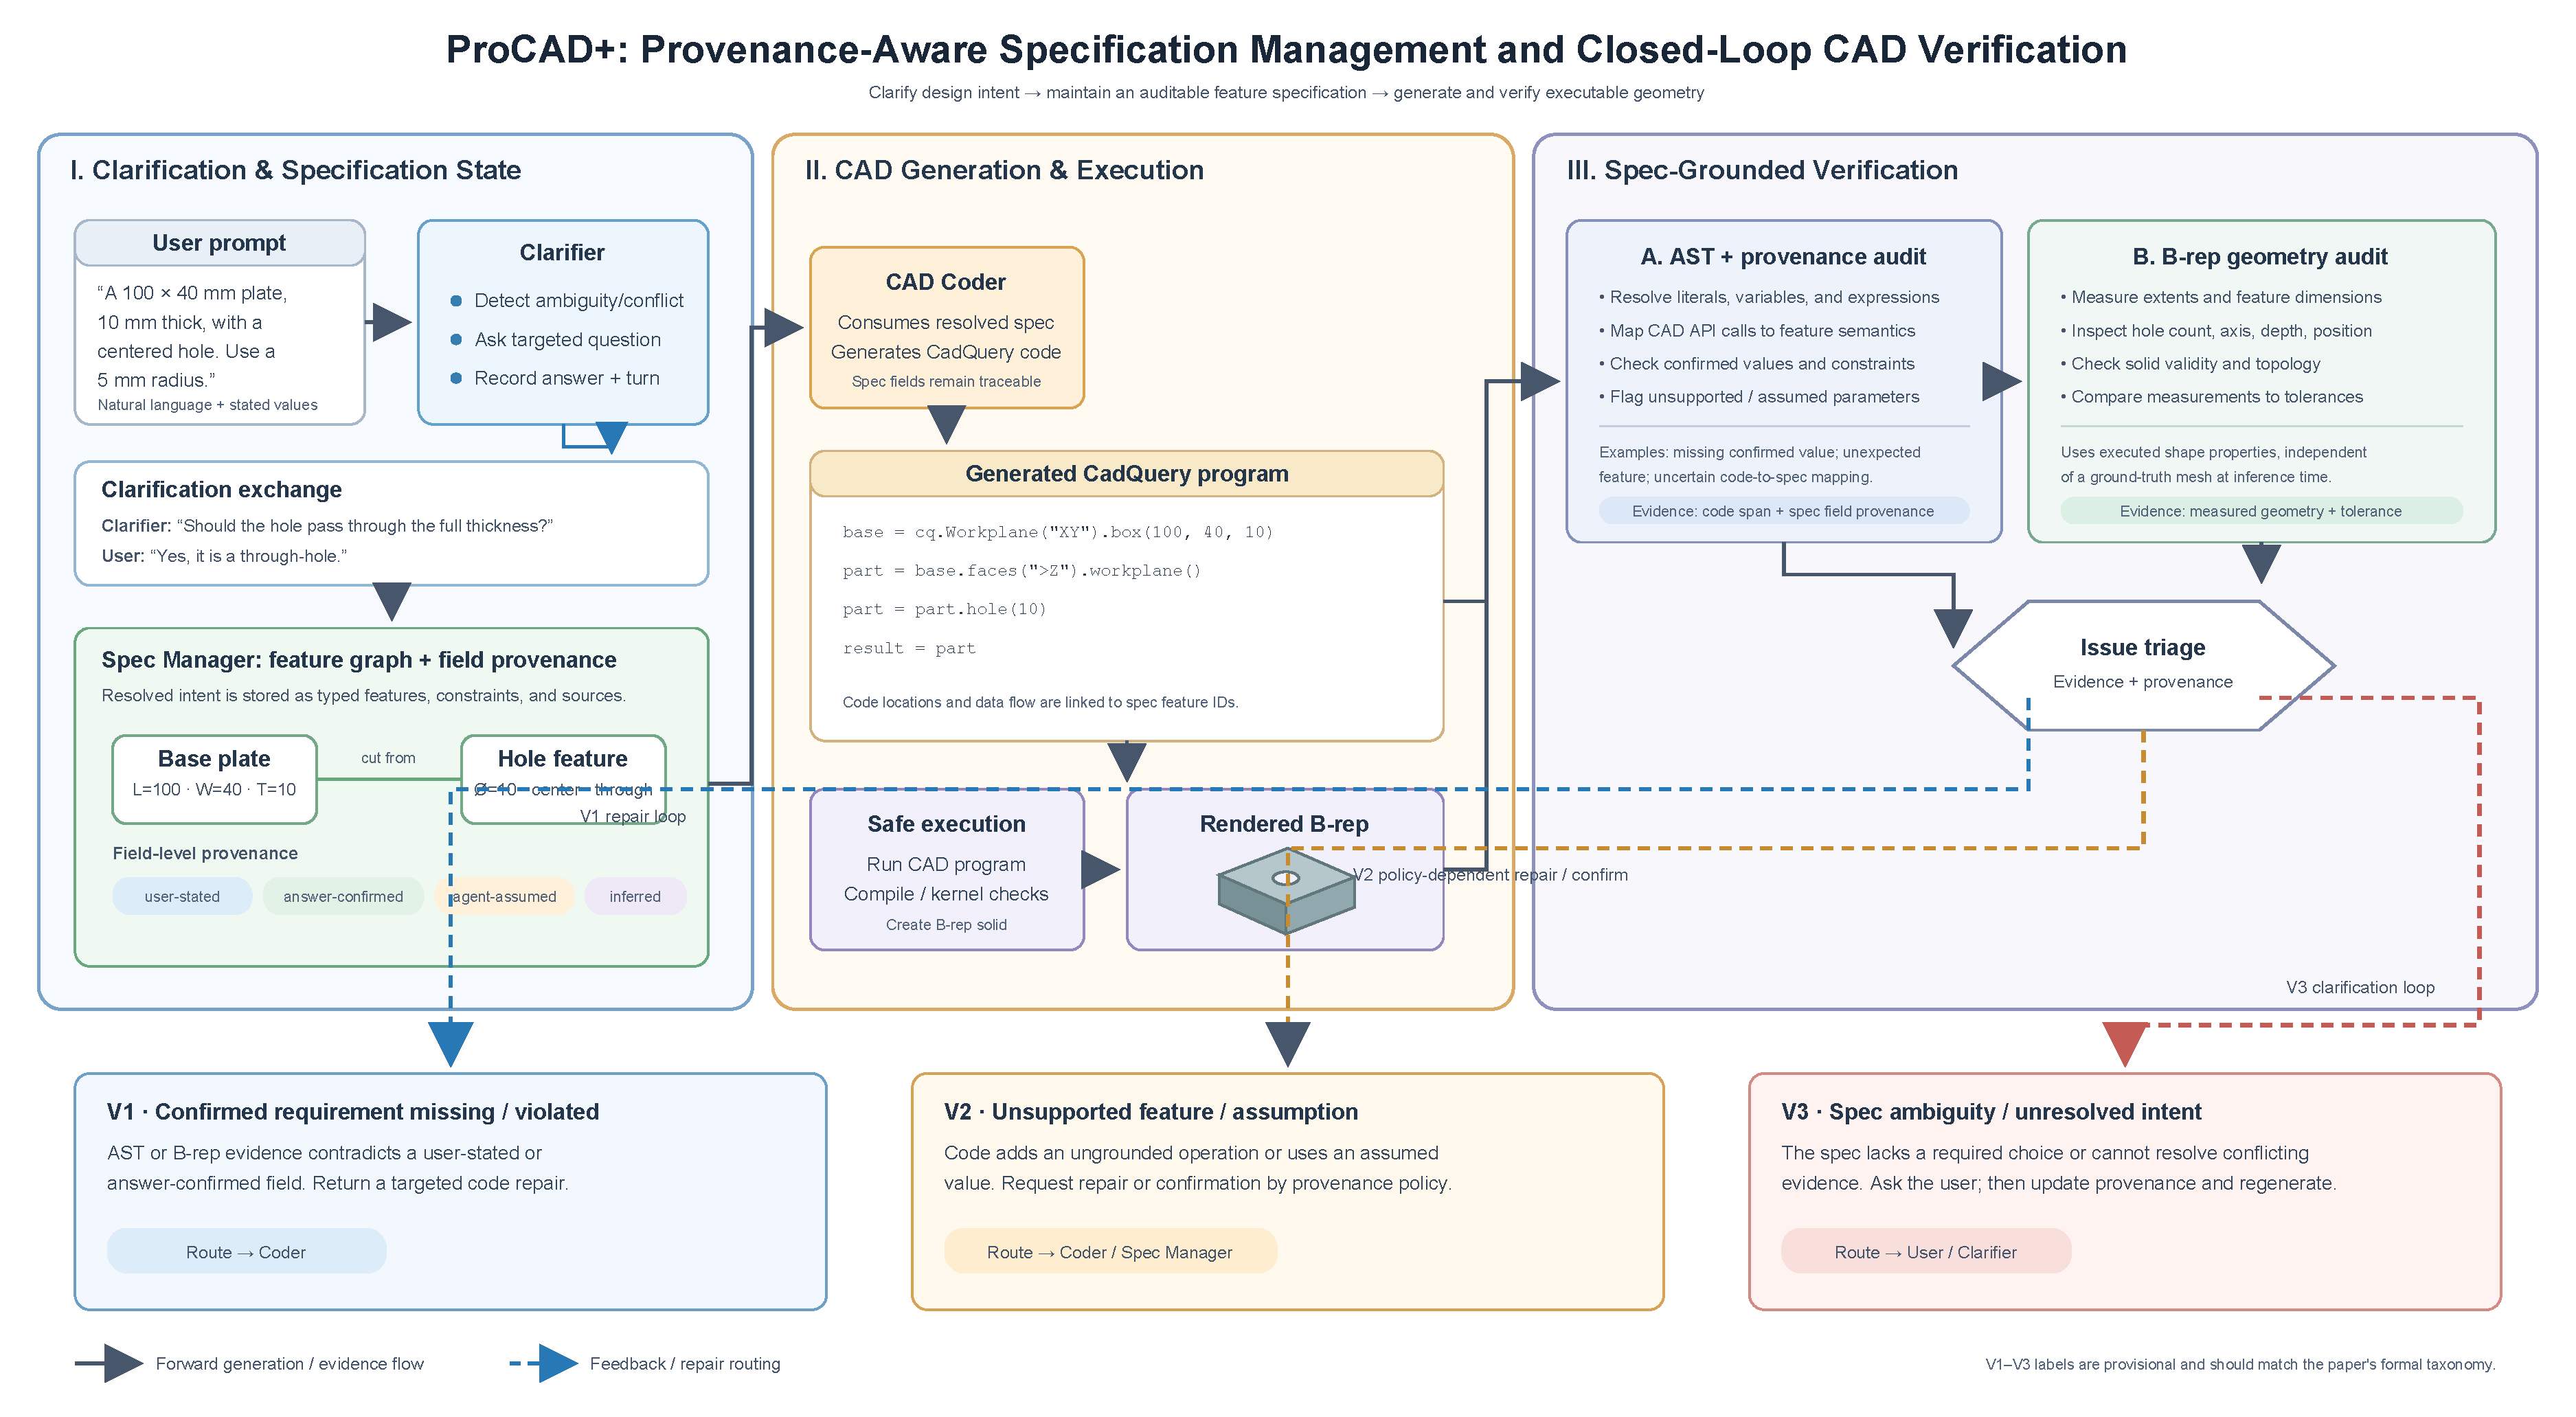
\includegraphics[width=\linewidth]{overview_figure.pdf}
  \caption{Pipeline overview. The specification is the single source of
  truth: it is grounded in the user's prompt and clarification answers,
  rendered for the coder, and used as the verification reference at
  deployment time, replacing the free-text hand-off and the ground-truth
  mesh.}
  \label{fig:overview}
\end{figure}

\section{Related Work}\label{sec:related}

\subsection{Text-to-CAD: from command sequences to executable programs}
\label{sec:related:t2c}

Learning-based CAD generation was first formulated as sequence modeling:
DeepCAD represents models as sketch-and-extrude command sequences and trains
a generative network over them \cite{deepcad}, and Text2CAD pairs such
sequences with natural-language descriptions at multiple levels of expertise
\cite{text2cad}. The shift to large language models recast CAD generation as
\emph{program synthesis}: LLM4CAD emits a Python-based domain-specific
language \cite{llm4cad}, Text-to-CAD aligns parametric data with language via
a vision--language model \cite{texttocad_vl}, and CAD-GPT augments multimodal
LLMs with spatial-reasoning prompts to synthesize construction sequences
\cite{cadgpt}. More recent systems generate directly executable CadQuery
programs and run them to obtain B-rep geometry \cite{procad,cadrille}.

Executable Python programs rather than opaque token vocabularies are now the
preferred target representation as well: CADRecode reverse-engineers point
clouds directly into CadQuery scripts with a small LLM and a
million-program synthetic corpus \cite{cadrecode}, and CADFS collects a
million-scale corpus of \emph{real} FeatureScript programs with complete
modeling histories, executes them through a CAD kernel to obtain B-reps, and
evaluates on Chamfer, normal consistency, and edge Chamfer distance
\cite{cadfs}; CAD-Llama adapts open-weight LLMs to the same
program-synthesis setting \cite{cadllama}. We adopt this executable-program
view---and CADFS's multi-metric evaluation, including edge-aware distances
that expose fine structural defects---but generate forward from language
while tracking where every required value came from.

Two further trends are directly relevant. First, \emph{structured
intermediate tokens help}: FlexCAD achieves controllable generation and
partial editing through hierarchy-aware masking of structured CAD text
\cite{flexcad}, and Pointer-CAD unifies B-rep and command sequences with
explicit pointer-based edge and face references \cite{pointercad}---structure
in the representation buys controllability that raw free text cannot. Second,
\emph{visual and geometric feedback during training helps the generator}:
CADFusion alternates between learning a visual-feedback model and fine-tuning
the LLM on that feedback \cite{cadfusion}, while FutureCAD grounds generated
programs onto text-described B-rep primitives and uses the grounding signal as
a reinforcement reward \cite{futurecad}. Crucially, both use feedback as a
\emph{training-time} signal over the generator; at inference time the user's
specification is still consumed once, as free text, with no record of which
values were stated, assumed, or corrected.

Multimodal unified representations such as CAD-MLLM \cite{cadmllm} and
general-purpose CAD agents that combine tools with vision--language models
\cite{caddesigner,cadassistant} broaden the range of solvable tasks, but do
not address the provenance and verification of the design requirements
themselves---the gap we target.

\subsection{Proactive clarification of user intent}\label{sec:related:clarify}

Rather than forcing a single prompt to carry every requirement, proactive
agents ask before acting; the idea appears in task-oriented dialogue and
information-seeking systems \cite{clarify_general} and, in CAD, is
instantiated by ProCAD \cite{procad}: a Clarifier detects underspecified or
conflicting prompts and asks targeted questions before a separately trained
Coder produces CadQuery. Misleading prompts---parameters removed
(underspecification) or duplicated with contradictory values (direct
conflict)---are synthesized at controlled severity $K$, and an oracle user
simulator answers from the ground-truth description. We build directly on
this problem formulation and reuse its benchmark protocol.

Our analysis, however, identifies a structural weakness: the two agents
exchange a single rewritten description with no schema, no per-parameter
provenance, and no post-generation check. Information lost in that rewrite is
unrecoverable downstream, and a wrong value carried through clarification is
undetectable without the ground-truth mesh that the benchmark happens to
provide. We replace the free-text hand-off with a provenance-tracked
specification, make the answering user explicitly imperfect in our
experiments, and add a verification loop the original pipeline lacks.

\subsection{Structured and editable intermediate representations}
\label{sec:related:structured}

Exposing intermediate structure has a long history in procedural and
constructive-solid-modeling systems, where CSG trees and feature histories
make geometry inspectable and locally editable
\cite{requicha,featurescript,openscad}. The recent generative literature
returns to this idea: CAD-Editor locates a target span in CAD text and
re-infills only that span, avoiding full re-generation for edits
\cite{cadeditor}; FlexCAD's hierarchy masking similarly preserves non-target
parts \cite{flexcad}.

Most directly related is Treellis \cite{treellis}, which has an LLM emit an
assembly modeling language (AML)---a CSG-style tree of primitives with
editable parameters---and presents the tree, viewport, and parameter panel as
linked, editable views; a scoped edit sends only the selected subtree to the
model. In a controlled study, structured editing largely eliminated the
``regenerate everything and watch unrelated parts change'' loop that plain
prompting produces. We take this as strong motivation that users and agents
alike need an intermediate object between language and geometry.

But Treellis's own measurements expose the other half of the problem: only 32
of 50 generated trees were editable on the first pass (43 with exemplars and
structural constraints), because nothing verifies that the tree faithfully
captures the intent or that its parameters are complete. Their tree is a
\emph{geometric} structure revealed after generation for a human to repair;
our specification is an \emph{intent} structure built before generation, with
every value attributed to a source, and checked by the agent itself without a
human in the loop. The two are complementary downstream: a
provenance-tagged specification is a natural authoring layer for an editable
assembly tree.

\subsection{Verifying and repairing generated programs}
\label{sec:related:verify}

Self-verification of LLM outputs ranges from consistency sampling
\cite{selfcheckgpt} and self-refinement \cite{selfrefine} to execution-based
repair, where compiler and runtime feedback drives another generation
attempt; in CAD, cadrille trains with online RL against execution feedback
\cite{cadrille}. The closest system, CADCodeVerify \cite{cadcodeverify},
prompts a VLM to (i) generate binary validation questions from the
description, (ii) answer them by looking at multi-view renders of its own
generated object, and (iii) rewrite code from the resulting feedback, with a
separate repair loop for compilation failures.

This verifies geometry \emph{visually and self-referentially}: the questions,
the answers, and the judged render all come from the same model, with no
grounded reference, and holistic image questions are insensitive to local
defects. SEEK-CAD applies the same render-and-critique loop with
chain-of-thought reasoning on open-weight models \cite{seekcad}, and ReCAD
improves the generator with reinforcement learning using visual feedback as
reward \cite{recad}; both inherit the unanchored, holistic nature of the
visual signal.

Closest to our goals is CADDesigner \cite{caddesigner}, a general-purpose
ReAct-style agent for conceptual CAD that combines three ingredients we also
rely on: a \emph{requirement-expansion} subagent that turns a vague request
into dimensions, constraints, assumptions, APIs, and an ordered modeling
process; an explicit-context imperative paradigm (ECIP) that keeps modeling
context and operation intent explicit during code generation; and iterative
repair driven by execution tracebacks and rendered visual feedback. It is,
to our knowledge, the clearest prior demonstration that surfacing an
intermediate structured representation and closing an execution loop
materially improves text-to-CAD. It differs from our method in the two
respects that define our contribution: the expanded requirement carries no
per-field provenance (stated vs.\ assumed is not recorded), and its repair
signal is the program's own execution error and self-rendered views---not a
check against the user-confirmed specification. CADDesigner is also a single
general-purpose agent; we argue in \S\ref{sec:discussion:agents} that a small
decomposition with a deterministic kernel is easier to verify than one
monolithic agent, a point we return to when discussing the number of agents.

A second family validates programs against geometry through the CAD kernel
itself, but in the \emph{reverse-engineering} setting where a target mesh is
available: CADFit casts mesh-to-CAD recovery as volumetric-IoU-guided
optimization over executable programs, pruning operations whose marginal IoU
contribution is non-positive and nearly eliminating invalid programs
\cite{cadfit}; StepCAD conditions an LLM policy on the current intermediate
geometry and performs test-time tree search with local program edits under an
IoU objective \cite{stepcad}. Kernel-executed validation and per-step
geometry conditioning are close in spirit to our dynamic B-rep checks, but
their reference signal is the \emph{target mesh being reverse-engineered}---
ground truth that exists offline in reconstruction and never exists when
generating from a user's description.

Our verifier is anchored instead to the explicit set of user-confirmed
parameters and is performed in two deterministic channels: static alignment
of program literals to specification fields, and direct measurement of the
executed B-rep (radii, depths, feature counts, topology), with a vision
channel reserved for semantics the measurements cannot cover. Failures are
routed by cause: an unconfirmed assumption triggers another clarification
question, while a confirmed value the coder dropped triggers a
diagnostic-grounded regeneration rather than another question. This is closer
in spirit to specification- and property-based program verification
\cite{propertytesting} than to visual self-critique, and it requires no
ground-truth mesh at inference---the reference geometry that offline Chamfer
evaluation depends on \cite{chamfer_evals}.

\subsection{Positioning}\label{sec:related:positioning}

Table~\ref{tab:positioning} summarizes the axes that matter. No prior
text-to-CAD system combines intent clarification with a provenance-tracked
hand-off representation; no prior CAD program verifier is anchored to
user-confirmed requirements rather than to a target mesh or an unanchored
visual self-check; and no prior pipeline routes verification failures back to
clarification or regeneration by failure type.

\begin{table*}[t]
  \centering
  \caption{Positioning against the closest systems. ``GT at inference''
  denotes whether the method consumes a reference geometry at deployment
  time (not during offline evaluation).}
  \label{tab:positioning}
  \small
  \resizebox{\textwidth}{!}{%
  \begin{tabular}{lccccc}
    \toprule
    System & Clarification & Hand-off repr. & Deployment-time verification & Closed loop & GT at inference \\
    \midrule
    Text2CAD / DeepCAD \cite{text2cad,deepcad} & -- & command sequence & -- & -- & -- \\
    ProCAD \cite{procad} & one round, oracle & free text & -- & -- & no \\
    CADFusion / FutureCAD \cite{cadfusion,futurecad} & -- & programs + grounding & training-time & training loop & no \\
    CADCodeVerify / SEEK-CAD \cite{cadcodeverify,seekcad} & -- & code + renders & visual self-Q\&A & verify$\to$rewrite & no \\
    CADFit / StepCAD \cite{cadfit,stepcad} & -- & executable programs & kernel/IoU vs.\ target & search & \emph{yes (recon.\ input)} \\
    CAD-Editor / FlexCAD \cite{cadeditor,flexcad} & -- & editable text & -- & partial edits & -- \\
    Treellis \cite{treellis} & -- & assembly tree (humans) & -- & human edits & no \\
    \textbf{Ours} & \textbf{on-demand, multi-round} & \textbf{provenance spec} & \textbf{AST + B-rep vs.\ spec} & \textbf{by failure type} & \textbf{no} \\
    \bottomrule
  \end{tabular}%
  }
\end{table*}

\section{Problem Formulation}\label{sec:formulation}

\paragraph{Setting.}
A user provides a description $x$ of a mechanical part. The description may
be \emph{underspecified} (parameters missing) or \emph{conflicting} (the same
feature given two incompatible values). A pipeline of agents must produce an
executable CadQuery program $c$ whose rendered geometry realizes the user's
intent, while spending at most a bounded number of clarification questions.

\paragraph{ProCAD protocol.}
We follow the ProCAD benchmark \cite{procad}. From a clean description
$x^\mathrm{orig}$ with ground-truth program and mesh, misleading variants are
synthesized at severity $K{\in}\{1,2,3\}$ by removing $K$ parameters
(\texttt{underspec}) or introducing $K$ contradictory values
(\texttt{conflict}). Each sample carries the ground-truth questions and
answers. Evaluation compares three conditions on identical samples:
$D_\mathrm{orig}$ (clean prompt, performance ceiling), $D_\mathrm{mis}$
(misleading prompt without clarification, the single-agent baseline), and
$D_\mathrm{clar}$ (misleading prompt after clarification), measured by
Chamfer distance to the ground-truth mesh and program validity.

\paragraph{Where the protocol is silent.}
The protocol measures \emph{geometric similarity to ground truth}, which
exists only offline. It says nothing about two deployment-time questions:
(Q1)~does the text handed to the coder faithfully represent what the user
stated and confirmed, and (Q2)~can the system itself detect failures without
the reference mesh? We formalize both.

\paragraph{Specification fidelity (Q1).}
Let $\mathcal{F}$ be the set of geometric facts (feature, parameter, value)
stated in the user's prompt or confirmed in clarification answers---the
\emph{grounded information set}. Let $h$ be the hand-off object the coder
receives. We distinguish three defect classes:
\begin{itemize}
  \item \textsc{Dropped}: a fact in $\mathcal{F}$ absent from $h$;
  \item \textsc{Unsupported}: a dimensional value in $h$ with no support in
  $\mathcal{F}$ (invented);
  \item \textsc{Carryover}: a wrong value introduced by the misleading
  prompt that survives into $h$ even though the correct value is in
  $\mathcal{F}$.
\end{itemize}
For free-text hand-offs, $h$ is a string and membership is decided by
fact-level audit; for our specification, both $\mathcal{F}$ and $h$ are
structured and the comparison is deterministic. \S\ref{sec:evaluation:defect}
reports defect rates per class and per severity.

\paragraph{Fidelity vs.\ similarity (Q2).}
We separate \emph{specification fidelity}---does program $c$ realize the
specification $s$ the user confirmed?---from \emph{geometric similarity}---
does the rendered geometry resemble a reference mesh? Similarity requires
ground truth and is measurable only offline; fidelity is decidable from
$(s,c)$ alone, hence at every run. The empirical claim this paper must defend
is that fidelity is a \emph{useful proxy}: interventions that raise fidelity
should raise similarity on the benchmark, and fidelity failures should
predict similarity failures. The evaluation
(\S\ref{sec:evaluation}) tests both directions.

\section{Method}\label{sec:method}

Our pipeline keeps the ProCAD stages---misleadingness detection, question
asking, answering, code generation---but replaces their connecting tissue.
Figure~\ref{fig:overview} shows the flow: a \emph{Spec Manager}
(\S\ref{sec:spec}) owns a structured specification built from the prompt and
clarification answers; the coder receives a rendering of that specification
(\S\ref{sec:handoff}); a \emph{spec-grounded verifier} (\S\ref{sec:verifier})
checks the generated program against the specification without ground truth;
and a routing policy (\S\ref{sec:loop}) closes the loop by failure type.

\subsection{Specification schema and provenance}\label{sec:spec}

\paragraph{Schema.}
The specification $s$ is a JSON object with a unit, a feature list, a
constraint list, and a change log:
\begin{equation*}
s = \langle \mathrm{unit},\ \{f_i\},\ \{c_j\},\ \{r_k\}\rangle,\qquad
f_i = \langle \mathrm{id},\ \mathrm{type},\ \mathrm{op},\ \theta_i\rangle
\end{equation*}
where each feature $f_i$ carries a stable identifier, a type from a fixed
vocabulary (plate, cylinder, hole, slot, chamfer, fillet, \dots), a
construction operation (add/subtract), and parameters $\theta_i$. Every
parameter entry is a tuple
$\langle \text{value},\text{unit},\text{source},\text{evidence}\rangle$,
where \textit{evidence} quotes the sentence that supports the value.

\paragraph{Provenance levels.}
The \textit{source} field takes four values, ranked:
\begin{center}
\small
\textsc{answer-confirmed} (4) $\succ$ \textsc{user-stated} (3) $\succ$\\
\textsc{inferred} (2) $\succ$ \textsc{agent-assumed} (1).
\end{center}
The ranking encodes the semantics of the misleading-prompt setting: a value
confirmed during clarification reflects the user's latest intent and
overrides an earlier (possibly wrong) statement; a default filled by the
system is the least trustworthy and must never silently overwrite either.

\paragraph{Deterministic kernel.}
All operations that must be \emph{correct} are implemented as pure functions
without any LLM call:
(i)~\texttt{normalize}, which coerces arbitrary model output into the
canonical schema---invalid provenance tags are demoted to
\textsc{agent-assumed}, bare values are wrapped into parameter entries, and
missing identifiers are assigned;
(ii)~\texttt{merge}, the provenance-ranked update rule below;
(iii)~\texttt{unresolved}, which lists required-but-missing or
assumed-but-unconfirmed parameters from a per-feature-type table of required
alternatives (e.g., a hole requires \textit{radius} or \textit{diameter},
plus \textit{depth} or \textit{through}); and
(iv)~\texttt{render}, the coder hand-off of \S\ref{sec:handoff}.
Because the kernel is pure, every invariant---provenance ranking, identifier
stability, resolution logging---is verified by offline unit tests.

\paragraph{Provenance-ranked merge.}
Given the current specification $s$ and a model-proposed update $s'$ (from
incorporating a question--answer round), the merged specification is computed
field by field. For a parameter present in both:
a higher-ranked source overrides a lower-ranked one;
equal rank with a changed value also overrides (a fresh statement wins);
equal value with higher rank upgrades the provenance tag only.
Every override where the old value differed appends a resolution record
$\langle \text{feature},\text{param},\text{old},\text{new},\text{source},
\text{evidence}\rangle$ to the change log---a machine-readable account of
\emph{where information changed}, which the verifier and the analysis in
\S\ref{sec:evaluation:defect} consume directly. Feature identity is matched by
identifier, with a same-type positional fallback that absorbs identifier drift
in model output. Corrections may mark features obsolete instead of deleting
them, so nothing confirmed ever disappears silently.

\subsection{The Spec Manager agent}\label{sec:specmanager}

The LLM performs exactly three \emph{perception} actions; everything else is
kernel:
\begin{enumerate}
  \item \textbf{Extract} ($x \mapsto s$): read a (possibly misleading)
  description and emit the specification, tagging what is literally written as
  \textsc{user-stated}---without silently correcting it---and preferring to
  omit a parameter over inventing one.
  \item \textbf{Incorporate} ($s, \mathrm{Q\&A} \mapsto s'$): apply a
  question--answer round; answers are authoritative and override conflicting
  user-stated values with \textsc{answer-confirmed} provenance and quoted
  evidence. The proposal $s'$ is then defensively reconciled by the
  deterministic merge, so a malformed or hallucinated update can only ever
  add \emph{lower}-ranked information.
  \item \textbf{Propose questions} ($s \mapsto q$): ask only about
  \texttt{unresolved} fields---one question per missing or assumed
  parameter, requesting a value with unit, or an explicit confirmation of an
  assumed default. If the LLM fails or hallucinates questions, a
  deterministic template generates them from the unresolved list, so every
  question is structurally grounded.
\end{enumerate}
Question rounds are driven by the specification state, not by free-form
detection: a sample whose specification has no unresolved fields consumes no
further questions, bounding interaction cost (\S\ref{sec:loop}).

\subsection{Coder hand-off}\label{sec:handoff}

The coder receives a rendering of the specification rather than a rewritten
prompt: each feature with its parameters, placement, and count; each
constraint; confirmed values tagged with their provenance; and assumed
values loudly marked (e.g., \texttt{[ASSUMED DEFAULT - NOT CONFIRMED BY
USER]}), so the coder can tell confirmed geometry from system defaults. The
same renderer with tags stripped is our \emph{no-provenance} ablation: an
identical structured document without source information, isolating the
contribution of provenance from that of structure alone.

\subsection{Spec-grounded verification without ground truth}
\label{sec:verifier}

The verifier answers one question: \emph{does the program realize the
specification the user confirmed?} It never sees the original prompt or any
reference mesh, and runs in two deterministic channels plus an optional
semantic one.

\paragraph{L1: static alignment.}
The program is parsed with a Python AST (never executed). Numeric literals
flowing into dimensional CadQuery calls (\texttt{box}, \texttt{circle},
\texttt{hole}, \texttt{extrude}, \texttt{chamfer}, \dots) are collected;
structural constants (0, 1, 90, 180, \dots), angle and count keywords are
excluded. The check is a code-to-spec field mapping, not mere presence of a
number: a literal grounds a value only through the call semantics and
argument position it appears in, and mappings the analysis cannot establish
reliably---computed expressions, aliased variables---yield an explicit
\textsc{Uncertain} verdict rather than a silent pass. Three verdicts result:
\begin{itemize}
  \item \textsc{ConfirmedValueMissing} (blocking): a user-stated or
  answer-confirmed value in $s$ has no reliably mapped literal in the
  program---the coder dropped or altered user intent. Radius\slash diameter
  duality is resolved in radial call contexts only.
  \item \textsc{UnsupportedLiteral} (warning): a dimensional literal in the
  program matches no specification value---the coder invented a dimension.
  \item \textsc{AssumedUsed}: an agent-assumed value is realized in the
  program. This is not a failure; it is the set of fields routed back for
  user confirmation.
\end{itemize}

\paragraph{L2: B-rep measurement.}
Numeric alignment cannot catch \emph{correct values with wrong operations}---
a hole that became a boss, a cut applied to the wrong face, a reversed
extrusion. The dynamic channel therefore executes the program and interrogates
the resulting B-rep through the CAD kernel: measured cylinder radii, extrusion
extents, feature counts, face and edge topology, volume, and bounding box are
compared against the specification fields, with per-field tolerances. This
turns the failure modes that defeat literal matching into measurable
discrepancies (e.g., subtract vs.\ add changes face count and volume while
leaving all literals grounded).

\paragraph{L3: optional semantic channel.}
A vision--language judge sees the specification and the program's multi-view
renders---not the original prompt---and is asked to confirm non-numeric
fields (feature types, boolean operations, placement). Its questions are
derived from specification fields, not freely generated, keeping even the
subjective channel anchored.

\paragraph{Why the anchor matters.}
Against a ground-truth mesh (Chamfer), the verifier checks the wrong thing
for deployment; against its own renders (visual self-Q\&A
\cite{cadcodeverify,seekcad}), it has no reference at all. Against the
confirmed specification, the check is objective, cheap, and available every
run. What the specification cannot express---intent the user never
stated---remains outside the verifier's reach by construction; we quantify
this boundary in \S\ref{sec:evaluation}.

\subsection{Closing the loop: routing by failure type}\label{sec:loop}

Verifier verdicts differ in \emph{what kind of failure} they indicate, and
are routed accordingly:
\begin{itemize}
  \item \textsc{AssumedUsed} $\to$ \textbf{re-clarify}: the information is
  genuinely missing from the specification; the Spec Manager asks the user,
  merges the answer, and the coder re-renders.
  \item \textsc{ConfirmedValueMissing} / \textsc{UnsupportedLiteral} $\to$
  \textbf{grounded re-generation}: the information exists and is confirmed;
  asking the user again would return the same answer. Instead the coder
  re-generates with a field-level diagnostic (``the specification
  requires hole\_1.radius = 5\,mm; it does not appear in your program''),
  targeting the failure without another interaction.
\end{itemize}
The loop runs at most once per sample; every artifact is logged---both
verification rounds, the route taken, the questions consumed. This
differential routing is what lets the closed loop compete at
\emph{equal question budgets} against pipelines that simply ask one more
unconditional round: re-clarification is spent only where information is
actually missing.

\section{Evaluation}\label{sec:evaluation}

The evaluation answers five questions. (E1)~Do free-text hand-offs lose
information measurably? (E2)~Does the provenance specification reduce those
defects, and does reducing them improve geometry? (E3)~Is the
deployment-time verifier a valid proxy for ground-truth geometric failure?
(E4)~Does the closed loop win at equal question budgets? (E5)~Does the
pipeline survive imperfect users and an open 7B Spec Manager?

\subsection{Setup}\label{sec:evaluation:setup}

\paragraph{Benchmark.}
We recreate the ProCAD benchmark: misleading variants at severity
$K{\in}\{1,2,3\}$ for both families (\texttt{underspec},
\texttt{conflict}), plus clean samples ($K{=}0$), each with
ground-truth questions, answers, program, and mesh.
\TODO{state sample counts per family and severity; confirm that baseline
numbers reproduce the released ProCAD checkpoints under our evaluation
settings; specify the question-budget accounting (what counts as a
question, per system); state that all systems are compared on identical
samples with identical Chamfer settings (8192 points, normalization,
thresholds).}

\paragraph{Systems.}
All systems share the same coder and test split; only the pre-code stages
differ:
\begin{itemize}\setlength\itemsep{0.1em}
  \item[\textbf{E0}] single coder, misleading prompt (single-agent baseline);
  \item[\textbf{E1}] ProCAD clarification, one round (original pipeline);
  \item[\textbf{E2}] Spec Manager, no verification loop, one unconditional
  extra question round (budget-matched control);
  \item[\textbf{E3}] full closed loop (verifier-triggered re-clarification /
  re-generation);
  \item[\textbf{E4}] E3 with provenance tags stripped (ablation:
  structure without provenance);
  \item[\textbf{E5}] E3 with the distilled Qwen2.5-7B Spec Manager replacing
  the teacher.
\end{itemize}

\paragraph{User conditions.}
Oracle (answers from ground truth, the original protocol), \emph{novice}
(approximate values, partial answers), and \emph{confused} (wrong values
confidently stated). The latter two use the ProCAD persona machinery on the
answering side, exposing the oracle assumption the original evaluation makes.

\paragraph{Metrics.}
Geometry: Chamfer distance (8192-point, normalized, the original protocol),
normal consistency (NC), edge Chamfer distance (ECD) \cite{cadfs}, volume
IoU, and program validity with failure-type classification (compile /
geometry / success). Defects: per-class rates of \textsc{Dropped},
\textsc{Unsupported}, \textsc{Carryover} (\S\ref{sec:formulation}) via a
deterministic numeric channel cross-checked by a fact-level LLM audit.
Interaction: questions and LLM calls per sample. Proxy validity:
precision\slash recall of verifier verdicts against a Chamfer failure threshold,
with a \RESULT{N}-sample human-labeled gold set for calibration.

\subsection{Results}\label{sec:evaluation:defect}

\paragraph{Hand-off defects exist and correlate with geometry.}
\RESULT{Table: defect rates per class and per $K$/family for E1 vs.\ E2/E3;
mean Chamfer of defective vs.\ clean samples.}

\paragraph{Provenance reduces defects and improves geometry.}
\RESULT{Table: E0--E5 $\times$ $\{$CD, NC, ECD, IoU, validity$\}$; the
four-quadrant report (spec-fail\slash CD-bad etc.) with the honest third quadrant.}

\paragraph{The verifier is a valid proxy.}
\RESULT{Table: verdict precision\slash recall vs.\ Chamfer-thresholded failure;
L1-only vs.\ L1+L2; the L2 contribution on the ``value-correct,
operation-wrong'' subset.}

\paragraph{Equal-budget comparison.}
\RESULT{Table: E3 vs.\ E2 at matched question budgets; questions-per-sample
distribution.}

\paragraph{Imperfect users and the open model.}
\RESULT{Table: oracle\slash novice\slash confused $\times$ $\{$E1, E3$\}$; E5 vs.\ E3
teacher-student gap; cost per sample.}

\subsection{Limitations}\label{sec:evaluation:limits}

The specification covers stated intent only; errors outside it (wrong global
topology the user never described) are invisible to the verifier and must
still be caught by similarity metrics offline. The feature-type vocabulary
bounds what the schema can express. On underspecified samples where the user
lawfully confirms values that differ from dataset ground truth, Chamfer
against the dataset mesh is not the right yardstick; we report
specification-grounded references for these cases
(\S\ref{sec:discussion}).

\section{Discussion and Conclusion}\label{sec:discussion}

\paragraph{Fidelity as a deployable signal.}
The paper's central empirical wager is that specification fidelity---cheap,
deterministic, and measurable on every run---tracks geometric correctness
closely enough to drive closed-loop intervention. The results above test the
wager in both directions: defect-reduction interventions improve
ground-truth metrics, and verifier verdicts predict geometric failures
without seeing any reference mesh.

\paragraph{Complementary interfaces.}
Treellis demonstrates the value of exposing editable structure to humans;
our specification is the agent-side counterpart, built before generation and
verified after it. The two compose naturally: a provenance-tagged
specification field is an ideal anchor for selecting the corresponding
subtree in an editable assembly view, and we view intent-level provenance
plus structure-level editing as the full-stack answer to the
``regenerate-everything'' pathology.

\paragraph{Honest boundaries.}
The verifier's reach ends where stated intent ends: unstated errors,
wrong topology never discussed with the user, and semantics beyond the
feature vocabulary remain the province of offline similarity metrics and,
eventually, human inspection. Under lawful non-uniqueness (underspecified
prompts with many valid resolutions), dataset-grounded Chamfer penalizes
valid confirmations; we therefore separate dataset-referenced scores from
specification-referenced ones rather than average over both.

\paragraph{On the number of agents.}
\label{sec:discussion:agents}
Our system has three agents---Clarifier, Spec Manager, and Coder---plus a
deterministic verifier that is a \emph{tool}, not an agent: it has no LLM, no
objectives, and no action choice. We deliberately stop at three. The
Clarifier and Coder are inherited from ProCAD and carry well-understood,
separately trained responsibilities; the Spec Manager is the single new
agent because it is the one component that genuinely needs state and
user-facing decisions---what to ask, which value to trust, where to route a
failure. The verifier stays a tool for a principled reason: a
specification--program checker is a total function, and naming it an agent
would invite exactly the ``multi-agent as prompt engineering'' criticism
that undermines the method's claim to verifiability. CADDesigner achieves a
comparable feature set inside one general-purpose agent \cite{caddesigner};
our ablation- and unit-test-friendly decomposition is an alternative whose
trade-off---more components, each with a smaller, mechanically checkable
contract---we argue is the right one when correctness, not fluency, is the
requirement. Three agents are also not a floor: a natural collapse is that
the Clarifier is eventually absorbed into the Spec Manager, whose
unresolved-field machinery already subsumes question asking, leaving a
two-agent system with the same guarantees. We leave that consolidation to
future work and report the three-agent form here because it isolates the
Spec Manager's contribution against the ProCAD baseline cleanly.

\paragraph{Conclusion.}
We replaced the last free-text hand-off in clarify-then-generate text-to-CAD
pipelines with a provenance-tracked specification governed by a deterministic
kernel, and grounded verification in what the user actually confirmed rather
than in ground-truth geometry or unanchored self-inspection. Information
loss, invention, and carried-over errors---invisible in free-text
pipelines---become measurable, preventable, and repairable at deployment
time, at question budgets matched to baselines, and reproducible on open
7B models throughout.

\paragraph{Reproducibility.}
All code (pipeline, deterministic kernel with offline unit tests, verifier,
distillation, and analysis scripts) and the SFT recipe are released; the
evaluation reuses the public ProCAD dataset and checkpoints.


\bibliographystyle{ACM-Reference-Format}
\bibliography{references}

\end{document}
